%==============================================================================
\chapter{Ergebnisse} \label{chap:ergebnis}
%==============================================================================

In diesem Kapitel werden die mit der vorgeschlagenen Modellierung berechneten Ergebnisse diskutiert. Dabei steht insbesondere die Frage im Fokus, ob die Modellierung den Leistungs- und Wärmebedarf der Kraftstoffsysteme akkurat vorhersagen kann. Hierfür wird die Methodik dieser Arbeit mit Daten aus der Literatur validiert. Danach wird im Rahmen einer Sensitivitätsanalyse die Auswirkung von Unsicherheiten der in Kapitel \ref{chap:param} bestimmten Parametern auf das Modellverhalten untersucht. Anschließend wird im Rahmen einer Parameterstudie analysiert, wie sich die Eintrittstemperaturen des Kraftstoffs in den ersten Wärmeübertrager und die Brennkammer auf die Modellierungen der Wasserstoff-Kraftstoffsysteme auswirkt. Abschließend erfolgt ein Vergleich des Leistungs- und Wärmebedarfs der Wasserstoff-Kraftstoffsysteme untereinander und mit dem Kerosin-Kraftstoffsystem anhand eines ausgewählten Betriebspunkts.

\section{Validierung}

Zur Validierung der Methodik dieser Arbeit wird das Wasserstoff-Kraftstoffsystem mit Pumpe angepasst, um das von Brewer \cite{Brewer.1991} vorgeschlagene Kraftstoffsystem nachzuempfinden. 

Folgende Modifikationen werden an der Modellierung vorgenommen: Die Druckverluste im rezirkulierten Kraftstoffstrom werden vernachlässigt. Eine parallele Wasserstoffverbrennung ist nicht vorgesehen. Der Wärmeeintrag des von Brewer vorgeschlagenen Rekuperators wird nicht berücksichtigt, da sich dieser Wärmeübertrager Stromabwärts der Entnahmestelle des rezirkulierten Kraftstoffs befindet - eine Konfiguration, die von der Modellierung dieser Arbeit abweicht. Um dennoch eine Vergleichbarkeit der Pumpenleistung zu gewährleisten, wird der Druckverlust dieses Wärmeübertragers zu den Druckverluste der Injektoren addiert. 

Ein weiterer Unterschied liegt in der Modellierung des Kraftstoffs: Während in dieser Arbeit Parawasserstoff verwendet wird, basieren Brewers Berechnungen auf Normalwasserstoff. Dies macht eine Anpassung der Modellparameter des Wasserstoff-Stoffmodels erforderlich. Tabelle \ref{Tab:brewer} zeigt die weiteren Änderungen der Parameter und Variablen gegenüber dem ursprünglichen Wasserstoff-Kraftstoffsystem mit Pumpe.

\begin{table}[ht]
    \centering
	\caption{Veränderte Parameter der Validierung}
	\begin{tabular} {|l|c|c|c|} \hline%
    \multicolumn{2}{|c|}{Parameter} & Einheit & Wert\\ \hline\hline%
    FOHE Druckverhältnis & $\pi_\mathrm{FOHE}$ & - & 1 \\ \hline
    Brennkammer-Massenstrom & $\dot{m}_\mathrm{BK}$ & kg/s & 0,166 \\ \hline
    Leitungsdruckverluste & $\Delta p_\mathrm{r}$ & kPa & 30 \\ \hline
    Injektordruckverluste & $\Delta p_\mathrm{inj}$ & kPa & 214,4 \\ \hline
    Brennkammerdruck & $p_\mathrm{BK}$ & kPa & 1516,2 \\ \hline
    Brennkammer-Eintrittstemperatur & $T_\mathrm{BK}$ & K & 264 \\ \hline
    Wärmeübertrager-Eintrittstemperatur & $T_\mathrm{W}$ & K & 200 \\ \hline
    \end{tabular}	
    \label{Tab:brewer}%
\end{table}
\FloatBarrier 

Tabelle \ref{Tab:validation} zeigt die von Brewer berechneten Werte und die mit der beschriebenen Methodik berechneten Werte. 

\begin{table}[ht]
    \centering
	\caption{Validierung der Methodik}
	\begin{tabular} {|l|c|c|c|c|c|} \hline%
    \multicolumn{2}{|c|}{Variable} & Einheit & Brewer \cite{Brewer.1991} & Diese Arbeit & Abweichung [\%] \\ \hline\hline%
    Pumpenleistung & $P_\mathrm{HP}$ & kW & 23,9 & 23,5 & -1,67 \\ \hline
    Wärme & $\dot{Q}$ & kW & 542,7 & 539,8 & -0,534 \\ \hline
    Rezirkulierter Massenstrom & $\dot{m}_\mathrm{R}$ & kg/s & 0,377 & 0,439 & +16,4 \\ \hline
    Pumpen-Austrittstemperatur & $T_{2,\mathrm{HP}}$ & K & 50 & 33,1 & -33,8 \\ \hline
    \end{tabular}	
    \label{Tab:validation}%
\end{table}
\FloatBarrier 

Die Werte für die Pumpenleistung und den Wärmebedarf stimmen mit Abweichung $<2\,\%$ weitgehend mit den Berechnungen von Brewer überein. Der berechnete rezirkulierte Massenstrom ist jedoch um $16,4\,\%$ größer, als der von  Brewer ermittelte Wert. Dies ist auf eine um $33,8\,\%$ geringere berechnete Pumpen-Austrittstemperatur zurückzuführen. Die Ursache dieser deutlichen Abweichung ist unklar. Aufgrund der geringen Unterschiede der zugeführten Wärme und der Pumpenleistung und somit in der Energiebilanz des Kraftstoffsystems, erscheint ein erheblicher Unterschied in den verwendeten Stoffmodellen unwahrscheinlich. Aufgrund dieser Problematik ist eine belastbare Validierung der Methodik dieser Arbeit nicht möglich.

\section{Sensitivitätsanalyse}

Im Folgenden wird eine Sensitivitätsanalyse durchgeführt und ausgewertet, um die für das Modellverhalten maßgeblichen Parameter zu identifizieren und die Auswirkungen der mit Unsicherheit behafteten Modellannahmen abzuschätzen. Zunächst werden hierfür die Unsicherheiten der Parameter geschätzt. Anschließend werden die mit Unsicherheit behafteten Parameter in die Modellierungen der Kraftstoffsysteme eingesetzt, um die Abweichungen der Leistungsbedarfe zu berechnen.

\subsection{Bestimmung der Schrittweiten}

Da die Parameterwerte keiner bekannten statistischen Verteilung folgen, sondern infolge ungenauer Annahmen abweichen können, werden die Schrittweiten der Parameter geschätzt. Für die Vorzeichen der jeweiligen Schrittweiten wird der pessimistische Fall angenommen. Die Änderung der Parameter resultiert also stets in einer erhöhten Pumpenleistung des Wasserstoff-Kraftstoffsystems mit Verdampfer.

Der Austrittsdruck der Niederdruckpumpe $p_\mathrm{LPFP}$ des Kerosin-Kraftstoffsystems ist stets höher als der Öldruck im Wärmeübertrager des Hauptölsystems und somit von diesem abhängig. Der Öldruck ist eine Funktion der Druckverlust des Ölsystems. Für den Parameter wird eine moderate Schrittweite von $-10\,\%$ gewählt.

Da die Druckverluste von Wärmeübertragern und Leitungen ein Auslegungsziel darstellen, sind sie nicht mit Unsicherheit behaftet. Jedoch können abweichende Anforderungen an das Gewicht dieser Komponenten eine Aufweichung der Auslegungsziele erfordern. Um diesen Effekt zu berücksichtigen werden der Leitungsdruckverlust $\Delta p_L$ und die Druckverluste $\pi_i$ der Wärmeübertrager mit einer Schrittweite von $+10\,\%$ variiert. Die Parameter werden hierfür in die Druckverluste $\Delta p_\mathrm{HP}$ (Wasserstoff-Kraftstoffsysteme) und $\Delta p_\mathrm{LP}$ (Kerosin-Kraftstoffsystem) zusammengefasst.

Die Unsicherheiten der verfügbaren Abwärme $\dot{Q}_\mathrm{FOHE}$ und den Injektor-Druckverlusten $\Delta p_\mathrm{inj}$ werden als gering eingeschätzt. Aus diesem Grund wird für diese Parameter eine Schrittweite von $\pm 5\,\%$ ausgewählt. Ähnliches gilt für die Wirkungsgrade der Pumpen und Verdichter. Für die Wirkungsgrade der Verdichter und der Hochdruckpumpe des Kerosin-Kraftstoffsystems wird eine absolute Schrittweite von $-0,04$ verwendet. Die Niederdruckpumpe des Kerosin-Kraftstoffsystems wird mit einer Schrittweite von $-0,03$ beaufschlagt. Aufgrund des geringen Wirkungsgrads der Hochdruckpumpe des Wasserstoff-Kraftstoffsystems, wird für ihren Wirkungsgrad eine Schrittweite von $-0,008$ verwendet.

\subsection{Auswertung der Sensitivitätsanalyse}

Auf Basis der zuvor bestimmten Schrittweiten wird im Folgenden die Sensitivität der Kraftstoffsysteme untersucht und ausgewertet. Zunächst werden die Ergebnisse der Modellierung des Wasserstoff-Kraftstoffsystems mit Verdampfer präsentiert. Daraufhin werden die Ergebnisse der Sensitivitätsanalysen der Wasserstoff-Kraftstoffsysteme miteinander verglichen. Abschließend werden die Ergebnisse der Sensitivitätsanalyse für das Kerosin-Kraftstoffsystem diskutiert. 

Die Ergebnisse der Sensitivitätsanalyse für das Wasserstoff-Kraftstoffsystem mit Verdampfer sind in Tabelle \ref{Tab:sensafter} dargestellt.

\begin{table}[ht]
	\centering
	\caption{Sensitivitätsanalyse des H$_2$-Kraftstoffsystems mit Verdampfer}
	\begin{tabular} {|l|c|c|c|c|c|} \hline%
		Parameter & Referenzwert & Einheit & Schrittweite & $ \Delta \sum P_i$ [\%] \\ \hline\hline%
		$\Delta p_\mathrm{HP}$ & 390 & \si{\kilo\Pa} & +39,0 & +4,11 \\ \hline 
		$\eta_\mathrm{HP}$ & 0,71 & - & -0,04 & +3,03 \\ \hline 
		$\eta_\mathrm{RV}$ & 0,71 & - & -0,04 & +1,97 \\ \hline 
		$\dot{Q}_\mathrm{FOHE}$ & 149 & \si{\kilo\W} & -7,45 & +0,0505 \\ \hline 
		$\Delta p_\mathrm{inj}$ & 169 & \si{\kilo\Pa} & +8,45 & +0,0827 \\ \hline 
	\end{tabular}	
	\label{Tab:sensafter}%
\end{table}
\FloatBarrier 

Mit einem Anstieg der Leistungen um  $4,11\,\%$ hat die Erhöhung der Druckverluste im Hochdrucksystem die größte Auswirkung auf die Verdichterleistungen des Wasserstoff-Kraftstoffsystems mit Verdampfer. Die Reduktion der Wirkungsgrade der Verdichter hat mit $3,03\,\%$ (Hochdruckverdichter) beziehungsweise $1,97\,\%$ (Rezirkulationsverdichter) eine moderate Auswirkung auf deren Leistungen.  

Die Auswirkungen der Variation der verfügbaren Abwärme und des Injektor-Druckverhältnisses auf die Verdichterleistungen sind vernachlässigbar gering.

Die Tabellen \ref{Tab:senspump} und \ref{Tab:sensdual} zeigen die Ergebnisse der Sensitivitätsanalysen für die Wasserstoff-Kraftstoffsysteme mit Hochdruckpumpe und Vormischung.

\begin{table}[ht]
	\centering
	\caption{Sensitivitätsanalyse des H$_2$-Kraftstoffsystems mit Pumpe}
	\begin{tabular} {|l|c|c|c|c|c|} \hline%
		Parameter & Referenzwert & Einheit & Schrittweite & $ \Delta \sum P_i$ [\%] \\ \hline\hline%
		$\Delta p_\mathrm{HP}$ & 390 & \si{\kilo\Pa} & +39,0 & +6,19 \\ \hline 
		$\eta_\mathrm{HP}$ & 0,154 & - & -0,008 & +1,47 \\ \hline 
		$\eta_\mathrm{RV}$ & 0,71 & - & -0,04 & +3,35 \\ \hline 
		$\dot{Q}_\mathrm{FOHE}$ & 149 & \si{\kilo\W} & -7,45 & +0,0511 \\ \hline 
		$\Delta p_\mathrm{inj}$ & 169 & \si{\kilo\Pa} & +8,45 & -0,054 \\ \hline 
	\end{tabular}	
	\label{Tab:senspump}%
\end{table}
\FloatBarrier 

\begin{table}[ht]
	\centering
	\caption{Sensitivitätsanalyse des H$_2$-Kraftstoffsystems mit Vormischung}
	\begin{tabular} {|l|c|c|c|c|c|} \hline%
		Parameter & Referenzwert & Einheit & Schrittweite & $ \Delta \sum P_i$ [\%] \\ \hline\hline%
		$\Delta p_\mathrm{HP}$ & 390 & \si{\kilo\Pa} & +39,0 & +4,06 \\ \hline 
		$\eta_\mathrm{HP}$ & 0,71 & - & -0,04 & +3,04 \\ \hline 
		$\eta_\mathrm{RV}$ & 0,71 & - & -0,04 & +1,92 \\ \hline 
		$\dot{Q}_\mathrm{FOHE}$ & 149 & \si{\kilo\W} & -7,45 & +0,051 \\ \hline 
		$\Delta p_\mathrm{inj}$ & 169 & \si{\kilo\Pa} & +8,45 & +0,084 \\ \hline 
	\end{tabular}	
	\label{Tab:sensdual}%
\end{table}
\FloatBarrier 

Die Wasserstoff-Kraftstoffsysteme weisen nur geringfügige Unterschiede in ihren Sensitivitäten auf. Das Wasserstoff-Kraftstoffsystem mit Hochdruckpumpe zeigt mit einer Steigerung der Gesamtleistung um $6,19\,\%$ eine besonders hohe Sensitivität gegenüber Erhöhungen der Druckverluste im Hochdrucksystem. Dies ist auf den hohen Anteil des Rezirkulationsverdichters an der Gesamtleistung zurückzuführen. Aus demselben Grund wirkt sich eine Änderung des Wirkungsgrads der Hochdruckpumpe prozentual geringer auf den gesamten Leistungsbedarf aus, als bei den Hochdruckverdichtern der anderen Wasserstoff-Kraftstoffsysteme. Die Sensitivitäten des Wasserstoff-Kraftstoffsystems mit Vormischung weichen kaum von denen des Wasserstoff-Kraftstoffsystems mit Verdampfer ab.

Die Ergebnisse der Sensitivitätsanalyse für das Kerosin-Kraftstoffsystem sind in Tabelle \ref{Tab:sensjeta} zusammengefasst.

\begin{table}[ht]
	\centering
	\caption{Sensitivitätsanalyse des Kerosin-Kraftstoffsystems}
	\begin{tabular} {|l|c|c|c|c|} \hline%
		Parameter & Referenzwert & Einheit & Schrittweite & $ \Delta \sum P_i$ [\%] \\ \hline\hline%
		$\Delta p_\mathrm{LP}$ & 115 & \si{\kilo\Pa} & +11,5 & +1,05 \\ \hline 
		$p_\mathrm{LP}$ & 930 & \si{\kilo\Pa} & -93,0 & +4,73 \\ \hline 
		$\eta_\mathrm{HP}$ & 0,73 & - & -0,04 & +4,29 \\ \hline 
		$\eta_\mathrm{LP}$ & 0,60 & - & -0,03 & +1,40 \\ \hline 
		$\dot{Q}_\mathrm{FOHE}$ & 112 & \si{\kilo\W} & -5,85 & -1,28 \\ \hline 
		$\Delta p_\mathrm{inj}$ & 300 & \si{\kilo\Pa} & +15,0 & +1,36 \\ \hline 
	\end{tabular}	
	\label{Tab:sensjeta}%
\end{table}
\FloatBarrier 

Das Kerosin-Kraftstoffsystem reagiert mit einer Steigerung der Pumpenleistungen von $1,05\,\%$ weniger sensitiv gegenüber Änderungen der Wärmeübertrager- und Leitungs-Druckverluste als die Modellierungen der Wasserstoff-Kraftstoffsysteme.

Zwar führt der verringerte Austrittsdruck zu einer geringeren Leistung der Niederdruckpumpe, jedoch steigt hierdurch das Druckverhältnis und die Leistung der Hochdruckpumpe. Die Auswirkungen auf die Hochdruckpumpe überwiegen, was zu einem Anstieg des Leistungsbedarfs um $4,73\,\%$ führt – der größten Abweichung unter den Parametern. 

Eine Verringerung des Wirkungsgrads der Hochdruckpumpe hat einen um $4,29\,\%$ höheren Leistungsbedarf zur Folge. Aufgrund des geringeren Leistungsbedarfs der Niederdruckpumpe hat die Variation ihres Wirkungsgrads mit $1,40\,\%$ eine geringere Auswirkung. 

Eine Steigerung der Injektor-Druckverluste führt zu einem um $1,36\,\%$ höheren Leistungsbedarf der Pumpen. 

Die verringerte Abwärme führt zu einem geringeren Massenstrom durch die Niederdruckpumpe und somit zu um $1,36\,\%$ verringerten Pumpenleistungen.

Für die Wasserstoff-Kraftstoffsysteme wurden die Druckverluste im Hochdrucksystem sowie die Wirkungsgrade der Verdichter als sensitive Parameter identifiziert. Aufgrund der ähnlichen Tendenzen ist eine Vergleichbarkeit der Ergebnisse der Wasserstoff-Kraftstoffsysteme untereinander trotz Abweichungen der Gesamtleistungen von bis zu $+6,19\,\%$ gewährleistet. Hingegen reagiert das Kerosin-Kraftstoffsystem besonders stark auf Änderungen des Austrittsdrucks der Niederdruckpumpe und des Wirkungsgrads der Hochdruckpumpe. Vergleiche zwischen den Wasserstoff-Kraftstoffsystemen und dem Kerosin-Kraftstoffsystem sind daher eingeschränkt möglich.

\section{Parameterstudie}

Um die Wechselwirkung zwischen Wärmeübertrager- und Brennkammer-Eintrittstemperatur auf die Wärme- und Leistungsbedarfe der Wasserstoff-Kraftstoffsysteme zu untersuchen wird eine zweidimensionale Parameterstudie durchgeführt. Dabei werden die Parameter und Konfiguration der Wasserstoff-Kraftstoffsysteme über den untersuchten Bereich als konstant angenommen. 

Eine Betrachtung der Wärmeübertrager-Eintrittstemperatur ist technisch wertvoll, da hohe Wärmeübertrager-Eintrittstemperaturen den Leistungsbedarf des Rezirkulationsverdichters steigern und somit den Gesamtwirkungsgrad des Triebwerks negativ beeinflussen können. Allerdings können je nach Auslegung der Wärmeübertrager hohe Eintrittstemperaturen erforderlich sein, um Vereisung zu verhindern. Da die Auswirkungen der Wärmeübertrager-Eintrittstemperatur auf den Leistungsbedarf mit der Brennkammer-Eintrittstemperatur gekoppelt sind, ist es sinnvoll, beide Parameter gemeinsam zu untersuchen. 

Da sich die Wasserstoff-Kraftstoffsysteme untereinander in ihrem Verhalten weitgehend ähneln, werden die Ergebnisse zunächst für die Architektur mit Hochdruckpumpe gezeigt. Anschließend werden die Unterschiede zwischen den Architekturen im Detail betrachtet.

\subsection{Architektur mit Hochdruckpumpe}

Abbildung \ref{fig:pumppower} zeigt den mechanischen Leistungsbedarf des Wasserstoff-Kraftstoffsystems mit Pumpe für den untersuchten Temperaturbereich. 

\begin{figure}[ht]
\centering
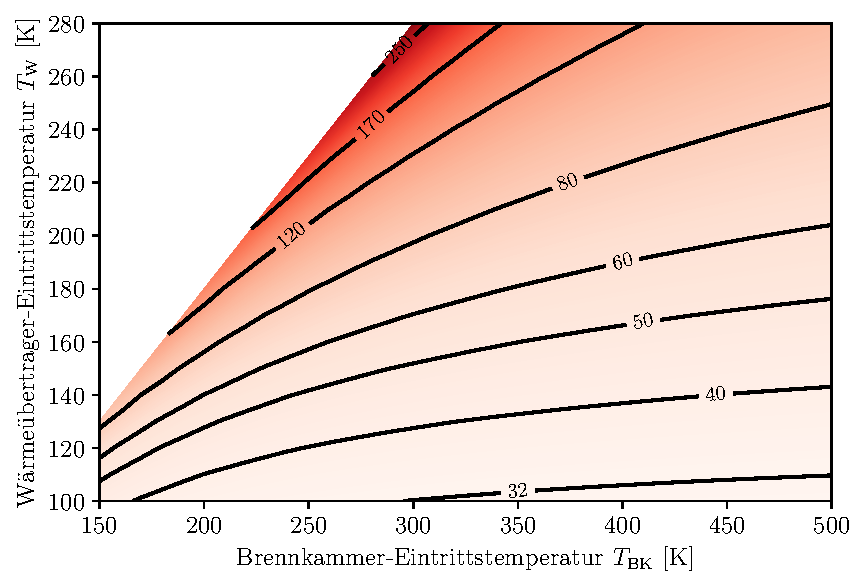
\includegraphics[width=0.95\linewidth]{4_Abbildungen/2_Hauptteil/Ergebnisse/Pumpepowercontour.pdf}
  \caption{Leistungsbedarf Wasserstoff-Kraftstoffsystem mit Pumpe}
  \label{fig:pumppower}
\end{figure}
\FloatBarrier

Der Gesamtleistungsbedarf $P$ steigt mit zunehmender Wärmeübertrager-Eintrittstemperatur, da eine geringe Differenz zur Brennkammer-Eintrittstemperatur einen größeren rezirkulierten Massenstrom erfordert, was die Leistung des Rezirkulationsverdichters erhöht. Zwar führen höhere Brennkammer-Eintrittstemperaturen zu einer Zunahme der spezifischen Arbeit des Rezirkulationsverdichters, jedoch wird dieser Effekt durch den reduzierten rezirkulierten Massenstrom mehr als ausgeglichen. Die Leistung der Hochdruckpumpe $P_\mathrm{HP}$ ist hingegen unabhängig von den Eintrittstemperaturen (Abbildung \ref{fig:pumpsplit}). 

\begin{figure}[ht]
\centering
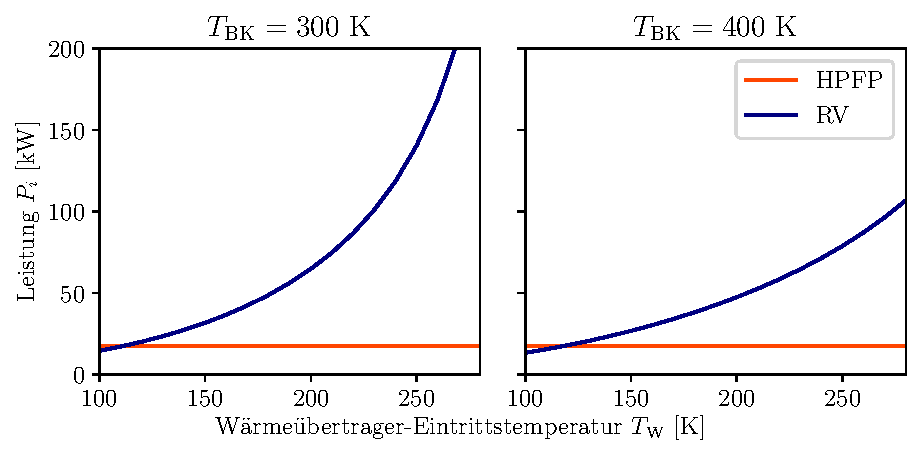
\includegraphics[width=1\linewidth]{4_Abbildungen/2_Hauptteil/Ergebnisse/Pumpe_powersplit.pdf}
  \caption{Leistungsaufteilung Wasserstoff-Kraftstoffsystem mit Pumpe}
  \label{fig:pumpsplit}
\end{figure}
\FloatBarrier

Der Wärmebedarf $\dot{Q}=\dot{Q}_\mathrm{FOHE}+\dot{Q}_\mathrm{PHC}$ ist insbesondere mit der Brennkammer-Eintrittstemperatur korreliert. Da die Leistung des Rezirkulationsverdichters $P_\mathrm{RV}$ mit steigender Wärmeübertrager-Eintrittstemperatur beziehungsweise geringer Differenz der Eintrittstemperaturen zunimmt, liegt in diesem Fall ein verringerter Wärmebedarf vor. Dieses Verhalten ist in Abbildung \ref{fig:pumpheat} dargestellt.

\begin{figure}[ht]
\centering
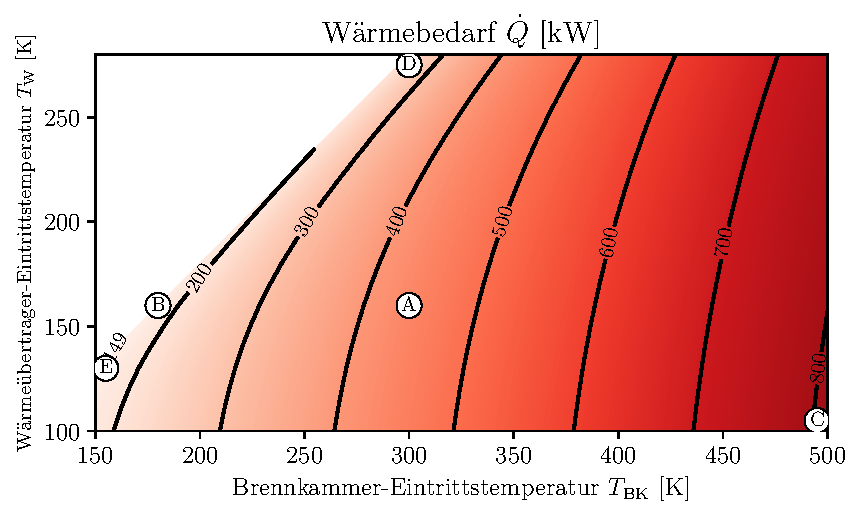
\includegraphics[width=1\linewidth]{4_Abbildungen/2_Hauptteil/Ergebnisse/Pumpeheatcontour.pdf}
  \caption{Wärmebedarf Wasserstoff-Kraftstoffsystem mit Pumpe}
  \label{fig:pumpheat}
\end{figure}
\FloatBarrier

Das Wasserstoff-Kraftstoffsystem erfordert fast über den gesamten betrachteten Temperaturbereich den Einsatz der parallelen Wasserstoffverbrennung. Lediglich in einem schmalen Bereich bei niedrigen Brennkammer-Eintrittstemperaturen (in der Abbildung links der \SI{149}{\kilo\W} Kontur) steht ausreichen Abwärme zur Verfügung.

Für die Bereitstellung der Wärme durch die parallele Wasserstoffverbrennung werden bis zu \SI{5.3}{\g\per\s} zusätzlichen Wasserstoff und \SI{0.53}{\kg\per\s} Fan-Zapfluft benötigt.


\subsection{Vergleich der Wasserstoff-Kraftstoffsysteme}

Im Folgenden werden die Ergebnisse der Parameterstudie der verschiedenen Wasserstoff-Kraftstoffsysteme miteinander verglichen. Abbildung \ref{fig:comp_power} zeigt den Leistungsbedarf der Kraftstoffsysteme in Abhängigkeit der Wärmeübertrager-Eintrittstemperatur für zwei verschiedene Brennkammer-Eintrittstemperaturen.

\begin{figure}[ht]
\centering
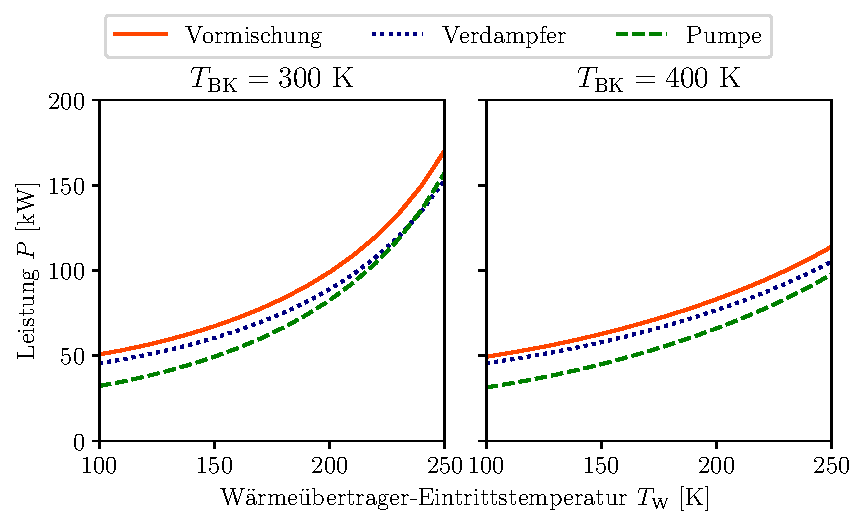
\includegraphics[width=0.9\linewidth]{4_Abbildungen/2_Hauptteil/Ergebnisse/summary_power.pdf}
  \caption{Gesamtleistungsbedarf Wasserstoff-Kraftstoffsysteme}
  \label{fig:comp_power}
\end{figure}
\FloatBarrier

Aufgrund der höheren spezifischen Arbeit der Verdichtung im gasförmigen Zustand weisen beide Kraftstoffsysteme mit Hochdruckverdichter im Vergleich zum Kraftstoffsystem mit Hochdruckpumpe einen erhöhten Leistungsbedarf auf. Da die Verdichter des Kraftstoffsystems mit Vormischung bei identischer spezifischer Arbeit einen größeren Massenstrom  fördern als die Verdichter der Architektur mit Verdampfer, hat das Kraftstoffsystem mit Vormischung einen höheren Leistungsbedarf. Dieser Effekt wird bei höheren Brennkammer-Eintrittstemperaturen abgeschwächt, da die Verdampfung in diesem Fall einen geringeren Massenstrom erfordert. Abbildung \ref{fig:comp_split} zeigt den Einfluss der Wärmeübertrager-Eintrittstemperatur auf die Komponenten-Leistungen.

\begin{figure}[ht]
\centering
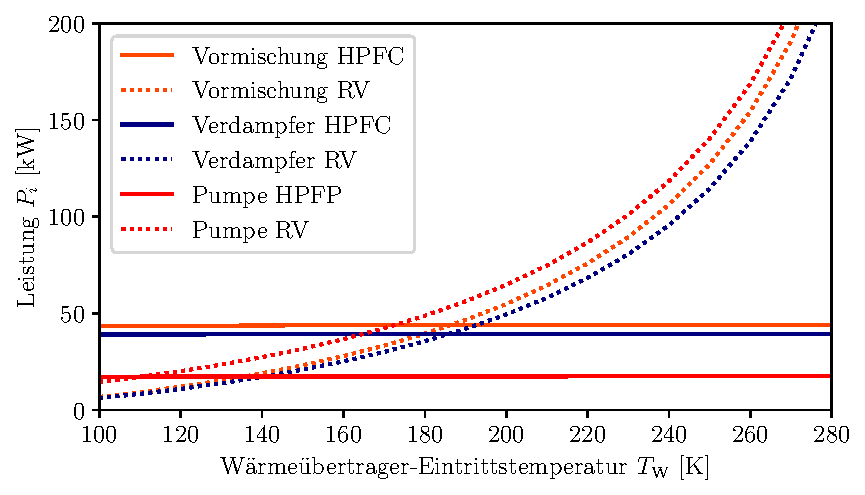
\includegraphics[width=0.85\linewidth]{4_Abbildungen/2_Hauptteil/Ergebnisse/300summary_powersplit.pdf}
  \caption{Leistungsaufteilung Vergleich Wärmeübertrager-Eintrittstemperatur}
  \label{fig:comp_split}
\end{figure}
\FloatBarrier

Analog zum Kraftstoffsystem mit Hochdruckpumpe hat die Wärmeübertrager-Eintrittstemperatur bei den Kraftstoffsystemen mit Hochdruckverdichter keinen Einfluss auf die Leistung des Hochdruckverdichters. Da die Kraftstoffsysteme mit Hochdruckverdichter im Vergleich zum Kraftstoffsystem mit Hochdruckpumpe einen geringeren rezirkulierten Massenstrom benötigen, fällt auch die Leistung des Rezirkulationsverdichters geringer aus. Abbildung \ref{fig:tbk_split} zeigt den Einfluss der Brennkammer-Eintrittstemperatur auf die Komponenten-Leistungen.

\begin{figure}[ht]
\centering
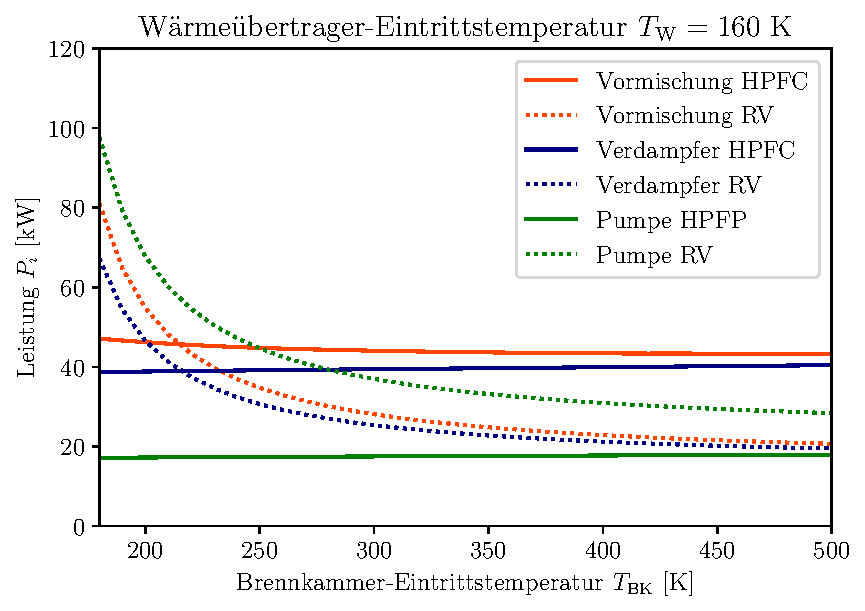
\includegraphics[width=0.9\linewidth]{4_Abbildungen/2_Hauptteil/Ergebnisse/tbkcomp.pdf}
  \caption{Leistungsaufteilung Vergleich Brennkammer-Eintrittstemperatur}
  \label{fig:tbk_split}
\end{figure}
\FloatBarrier

Der Trend sinkender Leistung des Rezirkulationsverdichters bei höherer Differenz der Eintrittstemperaturen setzt sich auch bei den Kraftstoffsystemen mit Hochdruckverdichter fort. Im Gegensatz zu den anderen Kraftstoffsystemen führen steigende Brennkammer-Eintrittstemperaturen bei dem Kraftstoffsystem mit Vormischung jedoch zu einer geringfügigen Reduzierung der Leistung des Hochdruckverdichters. Dies ist auf den geringeren erforderlichen Massenstrom für die Verdampfung zurückzuführen. 

Abbildung \ref{fig:stackplot} gibt einen Überblick der Leistungsanteile der Wasserstoff-Kraftstoffsysteme. In der linken Spalte sind die Leistungsanteile in Abhängigkeit der Brennkammereintritts-Temperatur bei konstanter Wärmeübertrager-Eintrittstemperatur dargestellt. Die mittlere Spalte zeigt die Leistungsanteile in Abhängigkeit der Brennkammer-Eintrittstemperatur, jedoch mit konstanter Temperaturdifferenz. Die rechte Spalte zeigt die Leistungsanteile in Abhängigkeit der Wärmeübertrager-Temperatur bei konstanter Brennkammereintritts-Eintrittstemperatur. Diese Abbildung verdeutlicht den Einfluss der Differenz der Eintrittstemperaturen. 

Bei einer konstanten Temperaturdifferenz von $T_{BK}-T_W=$ \SI{40}{\K} (mittlere Spalte) liegen die Leistung des Rezirkulationsverdichters $P_{RV}$ und die Wärme der parallelen Wasserstoffverbrennung $\dot{Q}_{PHC}$ über die untersuchten Brennkammer-Eintrittstemperaturen betragsmäßig in einem ähnlichen Bereich. Im Gegensatz dazu nimmt bei konstanter Brennkammer-Eintrittstemperatur der Leistungsanteil des Rezirkulationsverdichters mit steigender Wärmeübertrager-Eintrittstemperatur zu (rechte Spalte).

\begin{figure}[ht]
\centering
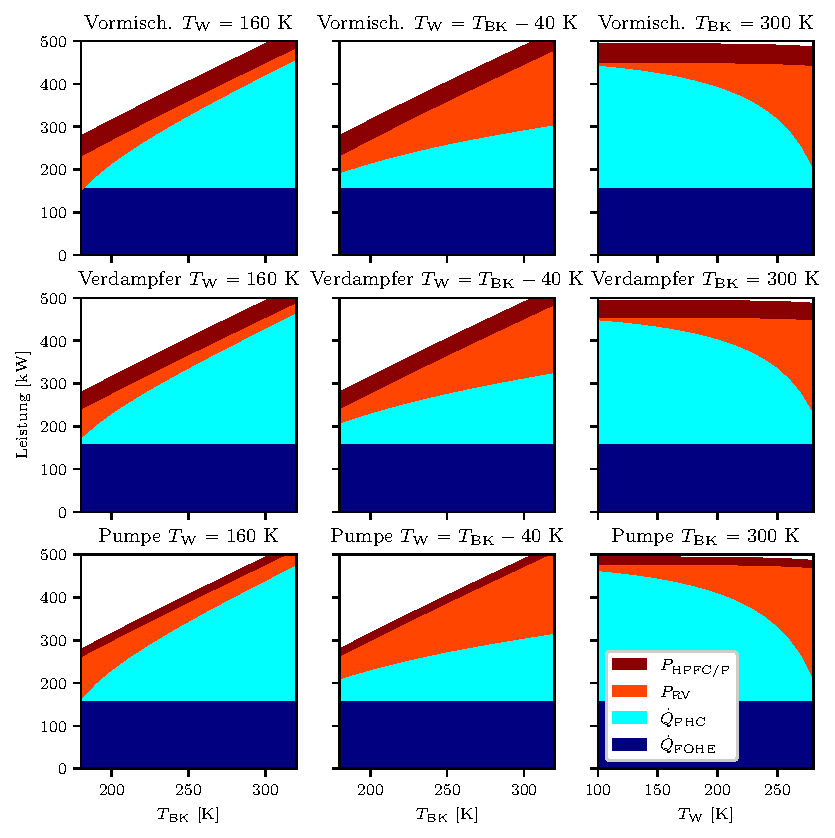
\includegraphics[width=1\linewidth]{4_Abbildungen/2_Hauptteil/Ergebnisse/stackplot_summary.pdf}
  \caption{Stapeldiagramme der Wärme-/Leistungsanteile}
  \label{fig:stackplot}
\end{figure}
\FloatBarrier

Eine direkte Empfehlung spezifischer Eintrittstemperaturen lässt sich aus diesen Daten nicht ableiten. Grundsätzlich gilt, dass entsprechend der technischen Möglichkeiten die Wahl einer möglichst niedrigen Wärmeübertrager-Eintrittstemperatur den Leistungsbedarf reduziert. Für die Brennkammer-Eintrittstemperatur lässt sich hingegen keine eindeutige Aussage treffen. Stattdessen sollte sie in Abhängigkeit von der Wärmeübertrager-Eintrittstemperatur gewählt werden.

\section{Vergleich Kerosin- und Wasserstoff-Kraftstoffsysteme}

Im Folgenden werden die Wasserstoff-Kraftstoffsysteme mit dem Kerosin-Kraftstoffsystem verglichen, um den abweichenden Bedarfe der betrachteten Systeme im Reiseflug zu verdeutlichen. 

Da die verfügbare Abwärme den Wärmebedarf des Kerosin-Kraftstoffsystems übersteigt, wird neben der in Kapitel \ref{chap:methodik} beschriebenen Berechnung, eine weitere Berechnung des tatsächliche Wärmebedarfs zum Erreichen der maximal zulässigen Brennkammer-Eintrittstemperatur durchgeführt. Hierfür wird der rezirkulierte Massenstrom $\dot{m}_\mathrm{R}$

\begin{equation}
	 \dot{m}_\mathrm{R}=\dot{m}_\mathrm{HP}-\dot{m}_\mathrm{BK} 
\end{equation}
 
so festgelegt, dass kein Kraftstoff in die Kraftstofftanks zurückgeführt wird. Die im Hauptölsystem-Wärmeübertrager zugeführte Wärme $\dot{Q}_\mathrm{FOHE}$ wird als Zielgröße modelliert und so angepasst, dass die maximal zulässige Brennkammer-Eintrittstemperatur $T_\mathrm{BK}$ gewahrt bleibt.

Abbildung \ref{fig:refcomp} zeigt den Wärme- und Leistungsbedarf der verschiedenen Kraftstoffsysteme. Für die Wasserstoff-Kraftstoffsysteme ist zudem der Wasserstoffbedarf der parallelen Wasserstoffverbrennung dargestellt. Für die Wasserstoff-Kraftstoffsysteme gilt eine Brennkammer-Eintrittstemperatur von $T_\mathrm{BK}=$ \SI{300}{\K} und eine Wärmeübertrager-Eintrittstemperatur von $T_\mathrm{W}=$ \SI{160}{\K}. Das Kerosin-Kraftstoffsystem erwärmt den Kraftstoff auf eine Brennkammer-Eintrittstemperatur von $T_\mathrm{BK}=$ \SI{399}{\K}.

\begin{figure}[ht]
\centering
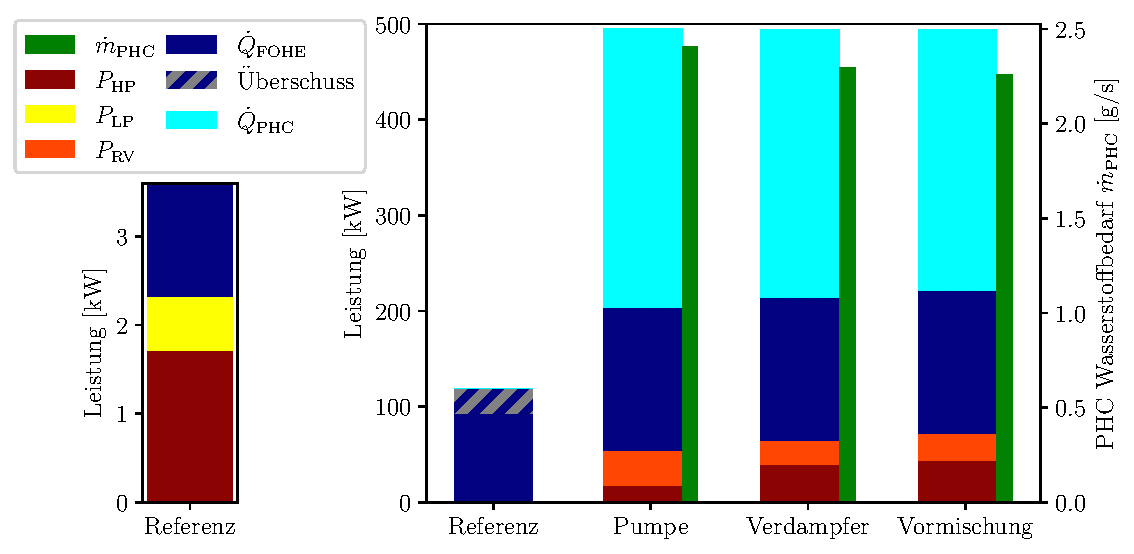
\includegraphics[width=1\linewidth]{4_Abbildungen/2_Hauptteil/Ergebnisse/refcomp.pdf}
  \caption{Bedarfe der Kraftstoffsysteme}
  \label{fig:refcomp}
\end{figure}
\FloatBarrier

Die Summe der Wärme- und Leistungsbedarfe der Wasserstoff-Kraftstoffsysteme übersteigen die des Kerosin-Kraftstoffsystems um einen Faktor von drei. Im Vergleich zum Kerosin-Kraftstoffsystem erfordert das Wasserstoff-Kraftstoffsystem mit Pumpe 23-Mal mehr Leistungsentnahme von der Hochdruckwelle und hat einen Wärmefehlbetrag von \SI{280}{\kilo\W}, der durch die parallele Wasserstoffverbrennung bereitgestellt wird. Bei dem Kraftstoffsystem mit Verdampfer wird sogar das 27-Fache an Leistungsentnahme benötigt bei einem Wärmefehlbetrag von \SI{270}{\kilo\W}. Bei dem Kraftstoffsystem mit Vormischung wird das 30-Fache an Leistungsentnahme benötigt bei einem Wärmefehlbetrag von nur noch \SI{260}{\kilo\W}. Die Bereitstellung der zusätzlichen Wärme durch die parallele Wasserstoffverbrennung verursacht einen zusätzlichen Wasserstoffbedarf von $\dot{m}_\mathrm{PHC}=2,2$ bis \SI{2.4}{\g\per\s}. Dies entspricht $2\,\%$ des Brennkammer-Massenstroms $\dot{m}_\mathrm{BK}$.

Von den \SI{117}{\kilo\W}, die dem Kerosin-Kraftstoffsystem an Abwärme zur Verfügung stehen, werden \SI{90}{\kilo\W} für die Erwärmung des Kraftstoffs benötigt. Um die überschüssigen \SI{27}{\kilo\W} durch Rückführung in die Kraftstofftanks zu kühlen, benötigt die Niederdruckpumpe zusätzliche Leistung in einer Höhe von \SI{0,14}{\kilo\W}. Dies entspricht $6\,\%$ der gesamten Pumpenleistungen des Kerosin-Kraftstoffsystems.

Die Abweichung der Leistungsbedarfe zwischen dem Kerosin- und den Wasserstoff-Kraftstoffsysteme übersteigt die Größenordnung der zuvor ermittelten Sensitivitäten um ein Vielfaches. Daher wird die Auswirkung fehlerbehafteter Annahmen auf das Vergleichsergebnis als unkritisch bewertet. 

